\subsection{信号的描述}

信号的描述有两种方式:数学描述和波形描述。

\begin{definition}[数学描述]
    信号的\bd{数学描述}是指,使用具体的数学表达式,
    把信号描述为一个或若干个自变量的函数或序列的形式。
\end{definition}

\begin{definition}[波形描述]
    信号的\bd{波形描述}是指,按照函数随自变量的变化关系,把信号的波形画出来。
\end{definition}

\begin{note}
    在画波形描述时,需要写清\bd{横纵坐标标识},并\bd{标出原点}。
\end{note}

\begin{example}
    以下是信号的数学描述和波形描述的例子:
    \begin{itemize}
        \item 数学描述:$f(t) = \sin t, x(n) = a^nu(n)$。
        \item 波形描述:$\sa(t) = \frac{\sin t}{t}$ 的示意图如图 \ref{fig:sa-t-wave-description}。
    \end{itemize}
    \begin{figure}[H]
        \centering
        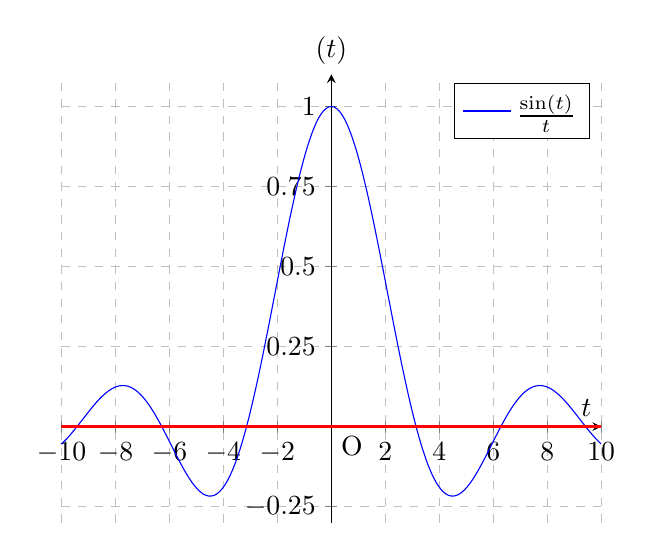
\begin{tikzpicture}
            \begin{axis}[
                axis lines = middle,
                xlabel = {$t$},
                ylabel = {$\sa(t)$},
                ylabel style={at={(rel axis cs:0.5, 1)}, anchor=south},
                xmin = -10, xmax = 10,
                ymin = -0.3, ymax = 1.1,
                xtick = {-10, -8, -6, -4, -2, 0, 2, 4, 6, 8, 10},
                ytick distance = 0.25,
                grid = major,
                grid style = dashed,
            ]
            \addplot[domain=-10:10, samples=100, smooth, blue] {sin(deg(x))/x};
            \addlegendentry{$\frac{\sin(t)}{t}$}
            \addplot[domain=-10:10, red, thick] {0};
            \node at (axis cs:0, 0) [anchor=north west] {O};
            \end{axis}
        \end{tikzpicture}
        \caption{$\sa(t) = \frac{\sin t}{t}$ 的波形描述}
        \label{fig:sa-t-wave-description}
    \end{figure}
\end{example}

\begin{example}[时域波形与频谱图]
    时域波形与频谱图如图 \ref{fig:wave-spectrum} 所示。
    \begin{figure}[H]
        \centering
        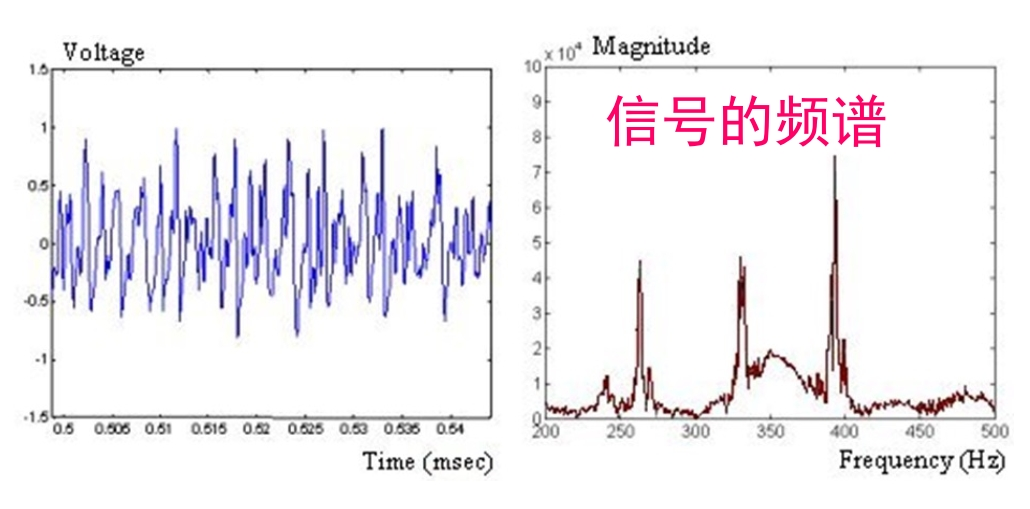
\includegraphics[width=0.5\textwidth]{chap1/img/wave-spectrum.png}
        \caption{左侧为时域波形,右侧为频谱图}
        \label{fig:wave-spectrum}
    \end{figure}
\end{example}

\begin{definition}[确定信号与随机信号]
    任意给定一个自变量的值,如果可以唯一确定其信号和取值,则该信号是\bd{确定信号}。
    否则,如果取值是不确定的随机值,则是\bd{随机信号}。
\end{definition}

\begin{definition}[周期信号]
    如果存在正数 $T$,使得对于任意 $t$ 都有 $f(t) = f(t + T)$,
    则称 $f(t)$ 为\bd{周期信号}。
    周期信号的\bd{周期} $T$ 是使得 $f(t) = f(t + T)$ 成立的最小正数。
\end{definition}

\begin{remark}
    非周期信号可以看做是周期为无穷大的周期信号。
\end{remark}

\begin{example}[正弦信号与余弦信号]
    正弦信号与余弦信号是最常见的周期信号。它们的数学描述如下:
    \begin{itemize}
        \item 正弦信号:$f(t) = K\sin(\omega t + \theta)$。
        \item 余弦信号:$f(t) = K\cos(\omega t + \theta)$。
    \end{itemize}
    其中 $K > 0$ 为振幅,$\omega$ 为角频率,$\theta$ 为初相位。
\end{example}

\begin{example}[$\sa$ 函数]
    $\sa$ 函数的数学描述如下:
    \begin{align*}
        \sa(t) = \frac{\sin t}{t}.
    \end{align*}
    它有以下性质:
    \begin{itemize}
        \item $\sa(t)$ 是偶函数。
        \item $\sa(t)$ 的零点为 $t = k\pi, k \ne 0$。
        \item 过零区间:除原点附近的过零区间宽度为 $2\pi$ 外,
            其他过零区间宽度均为 $\pi$。
        \item $\int_{-\infty}^{0}\sa(t)\D{t} = \int_{0}^{+\infty}\sa(t)\D{t} = \frac{\pi}{2}$,
            $\int_{-\infty}^{+\infty}\sa(t)\D{t} = \pi$。
    \end{itemize}
\end{example}

\begin{note}
    一定要注意,$\sa(t)$ 在 $t = 0$ 处的取值是 $1$,
    而不是 $0$。$\sa(t)$ 的零点不包括 $t = 0$。
\end{note}

\begin{example}[指数信号]
    指数信号是一种常见的非周期信号。它的数学描述如下:
    \begin{align*}
        f(t) = K\mathe^{\alpha t}.
    \end{align*}
    其中 $K > 0$ 为振幅,$\alpha$ 为参数。
    对于 $\alpha$ 的符号而言:
    \begin{itemize}
        \item 若 $\alpha > 0$,则信号随时间\bd{增强}。
        \item 若 $\alpha = 0$,则信号为\bd{直流信号}。
        \item 若 $\alpha < 0$,则信号随时间\bd{减弱}。
    \end{itemize}
    对于 $\alpha$ 的绝对值大小而言:
    \begin{itemize}
        \item 若 $\alpha$ 的绝对值大,则信号变化速度\bd{快}。
        \item 若 $\alpha$ 的绝对值小,则信号变化速度\bd{慢}。
    \end{itemize}
\end{example}

\begin{remark}
    指数信号微分或积分后仍然是指数信号。
\end{remark}
